\subsection*{Варьирование параметров -- агентная модель}
\addcontentsline{toc}{subsection}{Варьирование параметров -- агентная модель}

\textbf{Задание:}\\
Создать интерфейс модели SIR, позволяющий изменять количество агентов, параметры модели до запуска эксперимента. Создать эксперимент варьирования параметров. Визуализировать динамику инфицированных в зависимости от значения параметров.\\

\textbf{Решение:}\\
Изначально необходимо создать эксперимент варьирования параметров в окне проекта.\\

В качестве параметра варьирования был выбран параметр \textit{ProbInfection}, который отвечает за вероятность заражения индивида. (Рисунок \ref{fig:var_agent1})
\begin{figure}[h]
	\centering 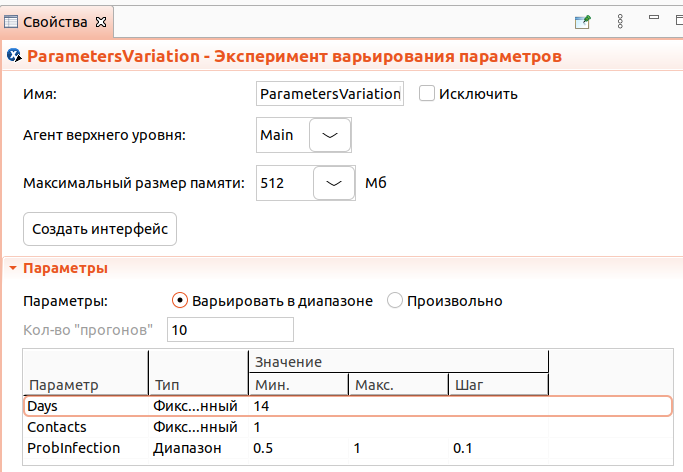
\includegraphics[scale=0.3]{var_agent1}
	\caption{Варьируемые параметры модели}
	\label{fig:var_agent1}
\end{figure}

Также необходимо создать интерфейс эксперимента. (Рисунок \ref{fig:var_agent2})
\begin{figure}[h]
	\centering 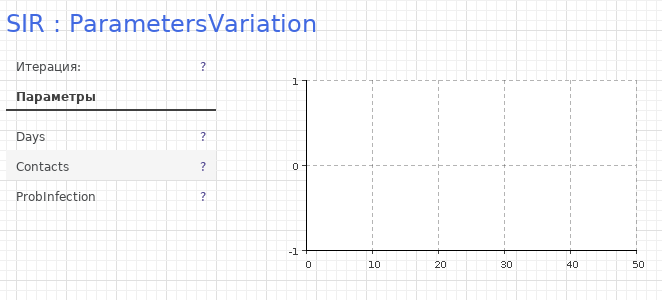
\includegraphics[scale=0.5]{var_agent2}
	\caption{Интерфейс варьирования эксперимента}
	\label{fig:var_agent2}
\end{figure}

\newpage

Данные для построения графиков берутся из статистики, в которой считается количество агентов, находящихся в состоянии -- инфицированных. (Рисунок \ref{fig:var_agent3})
\begin{figure}[h]
	\centering 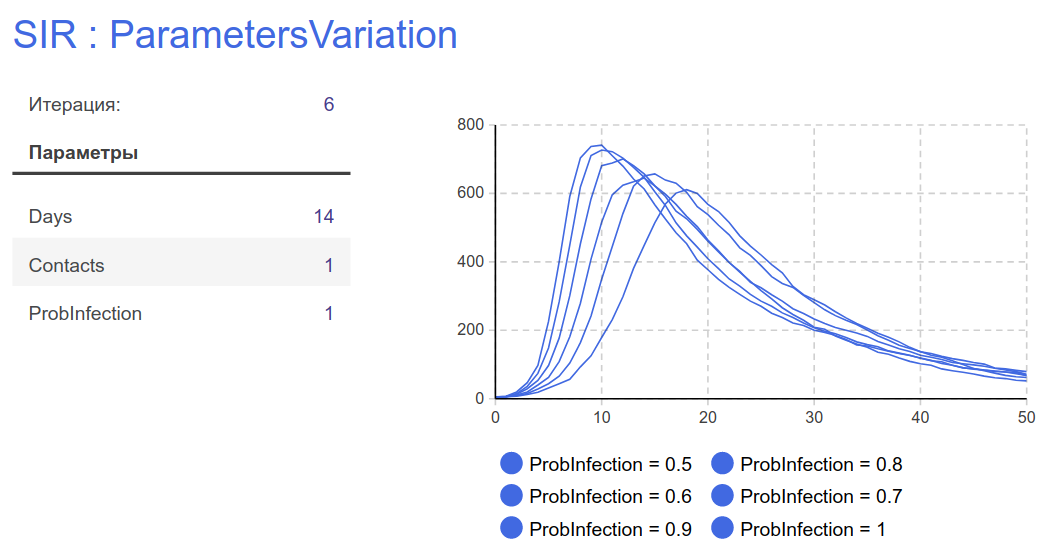
\includegraphics[scale=0.5]{var_agent3}
	\caption{Изменение объёма инфицированных людей}
	\label{fig:var_agent3}
\end{figure}

Таким образом, был создан эксперимент варьирования параметров для агентной модели, на примере которой были рассмотрены основные механики экспериментов варьирования параметров и их интерфейсов. 